\documentclass[11pt,a4paper]{article}

% Packages
\usepackage[margin=2.5cm]{geometry}
\usepackage{microtype}
\usepackage{graphicx}
\usepackage{tikz}
\usetikzlibrary{shapes,arrows.meta,positioning,calc,fit,backgrounds,shadows.blur,decorations.pathmorphing,decorations.pathreplacing}
\usepackage{colortbl}
\usepackage{enumitem}
\usepackage{booktabs}
\usepackage{longtable}
\usepackage{hyperref}
\usepackage{xcolor}
\usepackage{fancyhdr}
\usepackage{titlesec}
\usepackage[most]{tcolorbox}
\usepackage{multicol}
\usepackage{amsmath,amssymb}
\usepackage{multirow}
\usepackage{setspace}
\usepackage{fontawesome5}
\usepackage{listings}

% Spacing
\setlength{\parskip}{3pt plus 1pt minus 1pt}
\setlength{\parindent}{0pt}

% Colors
\definecolor{primary}{HTML}{1A5276}
\definecolor{secondary}{HTML}{2E86C1}
\definecolor{accent}{HTML}{E74C3C}
\definecolor{lightbg}{HTML}{EBF5FB}
\definecolor{defbg}{HTML}{FDF2E9}
\definecolor{greenhl}{HTML}{27AE60}
\definecolor{purplehl}{HTML}{8E44AD}
\definecolor{codebg}{HTML}{F4F6F7}

% Hyperref
\hypersetup{colorlinks=true, linkcolor=primary, urlcolor=secondary, citecolor=primary}

% Code listings style
\lstset{
  backgroundcolor=\color{codebg},
  basicstyle=\ttfamily\small,
  keywordstyle=\color{primary}\bfseries,
  stringstyle=\color{greenhl},
  commentstyle=\color{gray},
  breaklines=true,
  frame=l,
  framerule=2pt,
  rulecolor=\color{secondary!40},
  xleftmargin=8pt,
  framexleftmargin=6pt,
  aboveskip=6pt,
  belowskip=6pt,
  showstringspaces=false,
  language=Python
}

% Header/Footer
\pagestyle{fancy}
\fancyhf{}
\fancyhead[L]{\small\textcolor{primary}{\textbf{Natural Language Processing --- Core Concepts}}}
\fancyhead[R]{\small\textcolor{primary}{Lecture Handout}}
\fancyfoot[C]{\small\thepage}
\renewcommand{\headrulewidth}{0.5pt}
\renewcommand{\footrulewidth}{0.3pt}

% Section formatting
\titleformat{\section}{\Large\bfseries\color{primary}}{\thesection}{0.6em}{}[\vspace{2pt}\titlerule]
\titleformat{\subsection}{\large\bfseries\color{secondary}}{\thesubsection}{0.5em}{}
\titleformat{\subsubsection}{\normalsize\bfseries\color{primary}}{\thesubsubsection}{0.5em}{}
\titlespacing*{\section}{0pt}{14pt}{8pt}
\titlespacing*{\subsection}{0pt}{10pt}{5pt}

% Custom boxes
\newtcolorbox{definitionbox}[1][]{
  enhanced, breakable,
  colback=defbg, colframe=orange!60!black,
  colbacktitle=orange!70!black, coltitle=white,
  title={\faIcon{book}~#1}, fonttitle=\bfseries,
  boxrule=0pt, leftrule=4pt, arc=2pt,
  shadow={1mm}{-1mm}{0mm}{black!15},
  top=4pt, bottom=4pt, left=8pt, right=8pt
}
\newtcolorbox{conceptbox}[1][]{
  enhanced, breakable,
  colback=lightbg, colframe=secondary,
  colbacktitle=secondary, coltitle=white,
  title={\faIcon{lightbulb}~#1}, fonttitle=\bfseries,
  boxrule=0pt, leftrule=4pt, arc=2pt,
  shadow={1mm}{-1mm}{0mm}{black!15},
  top=4pt, bottom=4pt, left=8pt, right=8pt
}
\newtcolorbox{alertbox}[1][]{
  enhanced, breakable,
  colback=red!4, colframe=accent,
  colbacktitle=accent, coltitle=white,
  title={\faIcon{exclamation-triangle}~#1}, fonttitle=\bfseries,
  boxrule=0pt, leftrule=4pt, arc=2pt,
  shadow={1mm}{-1mm}{0mm}{black!12},
  top=3pt, bottom=3pt, left=8pt, right=8pt
}
\newtcolorbox{examplebox}[1][]{
  enhanced, breakable,
  colback=green!4, colframe=greenhl,
  colbacktitle=greenhl, coltitle=white,
  title={\faIcon{code}~#1}, fonttitle=\bfseries,
  boxrule=0pt, leftrule=4pt, arc=2pt,
  shadow={1mm}{-1mm}{0mm}{black!12},
  top=3pt, bottom=3pt, left=8pt, right=8pt
}

\begin{document}

% Title
\begin{center}
\vspace*{0.5cm}
{\Huge\bfseries\textcolor{primary}{Natural Language Processing}}\\[8pt]
{\Huge\bfseries\textcolor{primary}{Core Concepts Handout}}\\[16pt]
{\color{secondary}\rule{0.68\textwidth}{1.5pt}}\\[14pt]
{\Large\textsc{Summer 2026 --- BSIT, 3rd Semester}}\\[8pt]
{\large\textcolor{gray!70!black}{Foundations $\bullet$ Text Processing $\bullet$ Language Models $\bullet$ Representations $\bullet$ Retrieval $\bullet$ Sequence Models $\bullet$ Transformers $\bullet$ Speech $\bullet$ Ethics}}
\vspace{0.3cm}
\end{center}

\tableofcontents
\newpage

%=============================================================
\section{Introduction to Natural Language Processing}
%=============================================================

\begin{definitionbox}[Natural Language Processing]
Natural Language Processing (NLP) is the branch of Artificial Intelligence concerned with enabling computers to \textbf{read}, \textbf{understand}, \textbf{interpret}, and \textbf{generate} human language in a useful way, bridging human communication and machine computation.
\end{definitionbox}

\begin{conceptbox}[Why NLP Matters]
NLP powers search engines, machine translation, virtual assistants (Siri, Alexa), spam filters, chatbots, sentiment analysis for businesses, and modern large language models such as ChatGPT. For BSIT students, NLP skills are essential for building intelligent text- and speech-based applications.
\end{conceptbox}

\subsection{Why Language Is Hard for Machines}
\begin{itemize}[leftmargin=*]
  \item \textbf{Lexical Ambiguity:} A word has multiple meanings, e.g., ``bank'' (riverbank vs.\ financial bank).
  \item \textbf{Syntactic Ambiguity:} A sentence has more than one valid grammatical structure, e.g., ``I saw the man with the telescope.''
  \item \textbf{Semantic Ambiguity:} A sentence can have multiple possible meanings even with one structure.
  \item \textbf{Referential Ambiguity:} Pronouns can refer to more than one entity, e.g., ``Ali told John he passed the exam'' --- who passed?
  \item \textbf{Context Dependence:} Meaning often depends on world knowledge, tone, and prior conversation.
\end{itemize}

\subsection{A Brief History of NLP}
\begin{itemize}[leftmargin=*]
  \item \textbf{1950s:} Alan Turing's ideas and early rule-based machine translation experiments.
  \item \textbf{1960s--1980s:} Rule-based and grammar-based systems (e.g., the ELIZA chatbot, 1966).
  \item \textbf{1990s--2000s:} Statistical NLP --- probability and machine learning replace hand-written rules (n-gram models, Hidden Markov Models).
  \item \textbf{2010s:} Word embeddings (Word2Vec, GloVe) and deep learning (RNNs, LSTMs) transform NLP.
  \item \textbf{2017--present:} The Transformer architecture enables BERT, GPT, and modern Large Language Models (LLMs).
\end{itemize}

\subsection{Levels (Layers) of Language Analysis}
\begin{center}
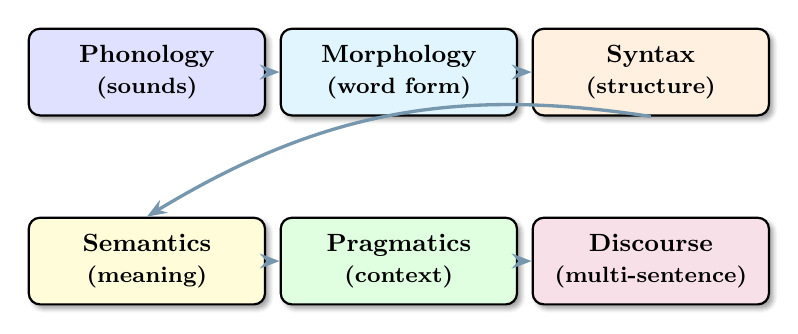
\begin{tikzpicture}[
  lvl/.style={rectangle, draw, thick, fill=#1, minimum width=3.0cm, minimum height=1.1cm, align=center, font=\small\bfseries, rounded corners=4pt,
    blur shadow={shadow blur steps=5, shadow xshift=0.5mm, shadow yshift=-0.5mm}},
  arr/.style={-{Stealth[length=2.5mm]}, very thick, primary!60, line width=1.2pt}
]
  \node[lvl=blue!12]   (p1) at (0,0)     {Phonology\\\footnotesize(sounds)};
  \node[lvl=cyan!12]   (p2) at (3.2,0)   {Morphology\\\footnotesize(word form)};
  \node[lvl=orange!12] (p3) at (6.4,0)   {Syntax\\\footnotesize(structure)};
  \node[lvl=yellow!15] (p4) at (0,-2.4)   {Semantics\\\footnotesize(meaning)};
  \node[lvl=green!12]  (p5) at (3.2,-2.4) {Pragmatics\\\footnotesize(context)};
  \node[lvl=purple!12] (p6) at (6.4,-2.4) {Discourse\\\footnotesize(multi-sentence)};
  \draw[arr] (p1) -- (p2);
  \draw[arr] (p2) -- (p3);
  \draw[arr] (p3.south) to[bend right=20] (p4.north);
  \draw[arr] (p4) -- (p5);
  \draw[arr] (p5) -- (p6);
\end{tikzpicture}
\end{center}

\begin{itemize}[leftmargin=*]
  \item \textbf{Phonology:} Sound patterns of language (relevant to speech recognition and synthesis).
  \item \textbf{Morphology:} Word structure and formation (prefixes, suffixes, roots).
  \item \textbf{Syntax:} Grammatical sentence structure.
  \item \textbf{Semantics:} Literal meaning of words and sentences.
  \item \textbf{Pragmatics:} Meaning in context (speaker intent, implication).
  \item \textbf{Discourse:} Meaning that spans multiple connected sentences.
\end{itemize}

%=============================================================
\section{The NLP Pipeline and Text Preprocessing}
%=============================================================

\begin{definitionbox}[Text Preprocessing]
Text preprocessing converts raw, messy text into a clean, structured form that NLP algorithms can work with, typically the very first stage of any NLP system.
\end{definitionbox}

\begin{center}
\begin{tikzpicture}[
  step/.style={rectangle, draw, thick, fill=#1, minimum width=2.3cm, minimum height=1.3cm, align=center, font=\footnotesize\bfseries, rounded corners=4pt,
    blur shadow={shadow blur steps=5, shadow xshift=0.5mm, shadow yshift=-0.5mm}},
  arr/.style={-{Stealth[length=2.5mm]}, very thick, primary!60, line width=1.2pt}
]
  \node[step=blue!12]   (s1) at (0,0)    {\faIcon{database}\\Raw\\Text};
  \node[step=cyan!12]   (s2) at (2.9,0)  {\faIcon{list-ol}\\Tokeniz-\\ation};
  \node[step=orange!12] (s3) at (5.8,0)  {\faIcon{broom}\\Cleaning /\\Normalization};
  \node[step=yellow!15] (s4) at (0,-2.5)   {\faIcon{cogs}\\Stemming /\\Lemmatization};
  \node[step=green!12]  (s5) at (2.9,-2.5) {\faIcon{brain}\\Feature\\Extraction};
  \node[step=purple!12] (s6) at (5.8,-2.5) {\faIcon{network-wired}\\Model /\\Task};
  \draw[arr] (s1) -- (s2);
  \draw[arr] (s2) -- (s3);
  \draw[arr] (s3.south) to[bend right=18] (s4.north);
  \draw[arr] (s4) -- (s5);
  \draw[arr] (s5) -- (s6);
\end{tikzpicture}
\end{center}

\subsection{Core Preprocessing Steps}
\begin{itemize}[leftmargin=*]
  \item \textbf{Tokenization:} Splitting text into smaller units --- words, sub-words, or sentences.
  \item \textbf{Lowercasing:} Converting all text to lowercase so ``Data'' and ``data'' are treated identically.
  \item \textbf{Stopword Removal:} Removing very common, low-information words (``the'', ``is'', ``and'').
  \item \textbf{Noise Removal:} Stripping punctuation, HTML tags, special characters, and extra whitespace.
  \item \textbf{Stemming:} Crudely chopping word endings using fixed rules (e.g., Porter Stemmer: ``studies'' $\to$ ``studi'').
  \item \textbf{Lemmatization:} Using vocabulary and grammar knowledge to return the correct dictionary root, or \textbf{lemma} (e.g., ``studies'' $\to$ ``study'', ``better'' $\to$ ``good'').
\end{itemize}

\rowcolors{2}{white}{defbg}
\begin{center}
\begin{tabular}{@{}p{2.6cm}p{5.3cm}p{5.3cm}@{}}
\toprule
\rowcolor{primary!15}
\textbf{Aspect} & \textbf{Stemming} & \textbf{Lemmatization} \\
\midrule
Approach & Rule-based suffix stripping & Dictionary and morphological analysis \\
Output & May not be a real word & Always a valid dictionary word \\
Speed & Faster, lightweight & Slower, needs vocabulary lookup \\
Accuracy & Lower, cruder & Higher, more linguistically correct \\
\bottomrule
\end{tabular}
\end{center}

\begin{examplebox}[Illustrative Example: Preprocessing a Sentence]
Raw text: \textit{``The Students are STUDYING Data Science!!!''}
\begin{itemize}[leftmargin=*]
  \item Tokenize: [The, Students, are, STUDYING, Data, Science, !, !, !]
  \item Lowercase + remove punctuation: [the, students, are, studying, data, science]
  \item Remove stopwords: [students, studying, data, science]
  \item Lemmatize: [student, study, data, science]
\end{itemize}
\end{examplebox}

%=============================================================
\section{Morphological and Lexical Analysis}
%=============================================================

\begin{definitionbox}[Morphology]
Morphology is the study of how words are formed from smaller meaningful units called \textbf{morphemes}, the smallest grammatical unit of a language.
\end{definitionbox}

\subsection{Types of Morphemes}
\begin{itemize}[leftmargin=*]
  \item \textbf{Free Morpheme:} Can stand alone as a word (e.g., ``book'', ``run'').
  \item \textbf{Bound Morpheme:} Cannot stand alone; must attach to another morpheme (e.g., ``-ing'', ``un-'', ``-s'').
  \item \textbf{Prefix / Suffix:} Bound morphemes attached before (``un-happy'') or after (``happy-ness'') a root word.
\end{itemize}

\subsection{Lexical Analysis and Vocabulary}
\begin{itemize}[leftmargin=*]
  \item \textbf{Lexicon:} The vocabulary of words (and their properties) known to an NLP system.
  \item \textbf{Out-of-Vocabulary (OOV) Words:} Words not seen during training, handled using sub-word tokenization (e.g., Byte-Pair Encoding) in modern systems.
  \item \textbf{Lexical Category:} The part of speech a word belongs to (noun, verb, adjective, etc.).
\end{itemize}

%=============================================================
\section{Regular Expressions and Finite-State Methods}
%=============================================================

\begin{definitionbox}[Regular Expression]
A regular expression (regex) is a compact pattern that describes a set of strings, widely used in NLP for tokenization, cleaning, and simple information extraction.
\end{definitionbox}

\subsection{Common Regex Building Blocks}
\rowcolors{2}{white}{defbg}
\begin{center}
\begin{tabular}{@{}p{2.6cm}p{4.6cm}p{5.2cm}@{}}
\toprule
\rowcolor{primary!15}
\textbf{Pattern} & \textbf{Meaning} & \textbf{Example Match} \\
\midrule
\texttt{[a-z]+} & One or more lowercase letters & ``hello'' \\
\texttt{\textbackslash d+} & One or more digits & ``2026'' \\
\texttt{\textasciicircum The} & Line starts with ``The'' & ``The dog ran'' \\
\texttt{cat|dog} & Either ``cat'' or ``dog'' & ``dog'' \\
\bottomrule
\end{tabular}
\end{center}

\begin{examplebox}[Illustrative Example: Extracting Years with Regex]
The pattern \texttt{\textbackslash d\{4\}} matches any 4-digit number. Applied to ``The event was held in 2023 and repeated in 2026'', it extracts \texttt{2023} and \texttt{2026} --- a simple, rule-based way to pull structured information from free text.
\end{examplebox}

\subsection{Finite-State Automata (FSA) for Morphology}
\begin{conceptbox}[FSA]
A Finite-State Automaton is a simple machine with a finite set of \textbf{states} and \textbf{transitions} triggered by input symbols. FSAs can compactly recognize valid word forms, e.g., accepting ``walk'', ``walks'', ``walked'', and ``walking'' but rejecting ``walkes''.
\end{conceptbox}
\begin{itemize}[leftmargin=*]
  \item Widely used for tokenization, morphological analysis, and spell-checking before statistical methods became dominant.
  \item Fast and predictable, but must be manually designed --- they do not learn from data like statistical or neural models.
\end{itemize}

%=============================================================
\section{Syntax and Parsing}
%=============================================================

\begin{definitionbox}[Syntax]
Syntax is the set of rules that govern how words combine to form grammatically correct sentences.
\end{definitionbox}

\subsection{Part-of-Speech (POS) Tagging}
\begin{conceptbox}[POS Tagging]
POS tagging assigns a grammatical category (noun, verb, adjective, determiner, etc.) to each word in a sentence, forming the basis for deeper syntactic and semantic analysis.
\end{conceptbox}
\textit{Example:} ``The/\textbf{DT} dog/\textbf{NN} barks/\textbf{VB} loudly/\textbf{RB}''

\subsection{Grammar and Parse Trees}
\begin{definitionbox}[Context-Free Grammar (CFG)]
A CFG defines valid sentence structures using production rules, e.g., $S \to NP\ VP$, $NP \to Det\ N$, $VP \to V$. Parsing uses these rules to build a \textbf{parse tree} showing a sentence's grammatical structure.
\end{definitionbox}

\begin{center}
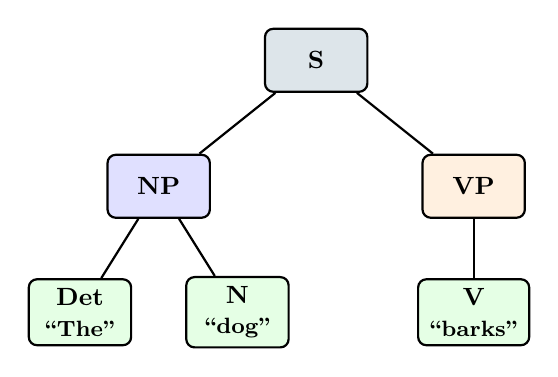
\begin{tikzpicture}[
  pnode/.style={rectangle, draw, thick, fill=#1, minimum width=1.3cm, minimum height=0.8cm, align=center, font=\small\bfseries, rounded corners=3pt}
]
  \node[pnode=primary!15] (s) at (0,0) {S};
  \node[pnode=blue!12] (np) at (-2,-1.6) {NP};
  \node[pnode=orange!12] (vp) at (2,-1.6) {VP};
  \node[pnode=green!10] (det) at (-3,-3.2) {Det\\\footnotesize``The''};
  \node[pnode=green!10] (n) at (-1,-3.2) {N\\\footnotesize``dog''};
  \node[pnode=green!10] (v) at (2,-3.2) {V\\\footnotesize``barks''};
  \draw[thick] (s) -- (np);
  \draw[thick] (s) -- (vp);
  \draw[thick] (np) -- (det);
  \draw[thick] (np) -- (n);
  \draw[thick] (vp) -- (v);
\end{tikzpicture}
\end{center}

\subsection{Constituency vs.\ Dependency Parsing}
\begin{itemize}[leftmargin=*]
  \item \textbf{Constituency Parsing:} Breaks a sentence into nested sub-phrases (as in the tree above), showing hierarchical grouping.
  \item \textbf{Dependency Parsing:} Shows grammatical relationships as directed links between individual words (e.g., ``barks'' is the root; ``dog'' is its subject), without grouping into phrases.
\end{itemize}

%=============================================================
\section{N-gram Language Models}
%=============================================================

\begin{definitionbox}[Language Model]
A language model assigns a probability $P(w_1, w_2, \ldots, w_n)$ to a sequence of words, capturing how likely that sequence is to occur in natural language.
\end{definitionbox}

\subsection{The Chain Rule and the Markov Assumption}
By the chain rule of probability:
$$
P(w_1,\ldots,w_n) = \prod_{i=1}^{n} P(w_i \mid w_1,\ldots,w_{i-1})
$$
Computing this exactly needs impossibly large amounts of data, so n-gram models make the \textbf{Markov assumption}: a word depends only on the previous $n-1$ words. For a \textbf{bigram} model ($n=2$):
$$
P(w_1,\ldots,w_n) \approx \prod_{i=1}^{n} P(w_i \mid w_{i-1}), \qquad
P(w_i\mid w_{i-1}) = \frac{\text{Count}(w_{i-1}, w_i)}{\text{Count}(w_{i-1})}
$$

\subsection{Smoothing}
\begin{conceptbox}[Why Smoothing Is Needed]
If a bigram never appeared in training data, its raw probability is zero --- which would make the whole sentence probability zero. \textbf{Smoothing} reserves a small amount of probability mass for unseen events.
\end{conceptbox}
Laplace (add-one) smoothing:
$$
P_{\text{Laplace}}(w_i\mid w_{i-1}) = \frac{\text{Count}(w_{i-1},w_i)+1}{\text{Count}(w_{i-1})+V}
$$
where $V$ is the vocabulary size.

\begin{conceptbox}[Beyond Laplace Smoothing]
More advanced techniques such as \textbf{Good-Turing smoothing} (re-estimates probabilities using the count of counts) and \textbf{Kneser-Ney smoothing} (accounts for how many different contexts a word appears in) generally perform better than simple add-one smoothing in real language models.
\end{conceptbox}

\subsection{Perplexity}
\begin{definitionbox}[Perplexity]
Perplexity measures how well a language model predicts a test sequence $W$ of $N$ words --- \textbf{lower perplexity means a better model}:
$$
PP(W) = P(w_1,\ldots,w_N)^{-\frac{1}{N}}
$$
\end{definitionbox}

%=============================================================
\section{Text Representation Techniques}
%=============================================================

\begin{definitionbox}[Text Representation]
Since machine learning models require numbers, text must be converted into numerical vectors before it can be processed --- this is called \textbf{text representation} or \textbf{feature extraction}.
\end{definitionbox}

\subsection{One-Hot Encoding and Bag-of-Words}
\begin{itemize}[leftmargin=*]
  \item \textbf{One-Hot Encoding:} Represents each word as a vector of zeros with a single 1 at that word's position in the vocabulary. Vectors are large and carry no notion of similarity.
  \item \textbf{Bag-of-Words (BoW):} Represents a document as a vector of word counts, ignoring word order and grammar.
\end{itemize}

\subsection{TF-IDF}
\begin{definitionbox}[TF-IDF]
Term Frequency--Inverse Document Frequency weighs a term by how often it appears in a document, offset by how common it is across all documents --- so common words get lower weight and distinctive words get higher weight.
$$
TF(t,d) = \frac{\text{count of } t \text{ in } d}{\text{total terms in } d}, \qquad
IDF(t) = \log\frac{N}{df_t}, \qquad
TF\text{-}IDF(t,d) = TF(t,d)\times IDF(t)
$$
where $N$ is the total number of documents and $df_t$ is the number of documents containing term $t$.
\end{definitionbox}

\subsection{Word Embeddings}
\begin{conceptbox}[Word Embeddings]
Word embeddings represent each word as a dense, low-dimensional vector learned from large text corpora, such that words with similar meanings have similar vectors (e.g., Word2Vec, GloVe).
\end{conceptbox}
\begin{itemize}[leftmargin=*]
  \item \textbf{CBOW (Continuous Bag of Words):} Predicts a target word from its surrounding context words.
  \item \textbf{Skip-gram:} Predicts the surrounding context words from a single target word.
  \item \textbf{Analogy Property:} Embeddings can capture relationships, famously $\text{king} - \text{man} + \text{woman} \approx \text{queen}$.
\end{itemize}

\begin{center}
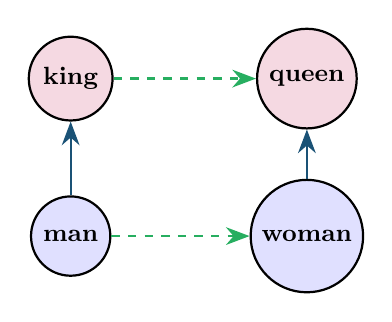
\begin{tikzpicture}
  \node[circle, draw, thick, fill=purple!15, minimum size=0.9cm, font=\small\bfseries] (king) at (0,2) {king};
  \node[circle, draw, thick, fill=purple!15, minimum size=0.9cm, font=\small\bfseries] (queen) at (3,2) {queen};
  \node[circle, draw, thick, fill=blue!12, minimum size=0.9cm, font=\small\bfseries] (man) at (0,0) {man};
  \node[circle, draw, thick, fill=blue!12, minimum size=0.9cm, font=\small\bfseries] (woman) at (3,0) {woman};
  \draw[-{Stealth[length=3mm]}, thick, primary] (man) -- (king);
  \draw[-{Stealth[length=3mm]}, thick, primary] (woman) -- (queen);
  \draw[-{Stealth[length=3mm]}, thick, dashed, greenhl] (man) -- (woman);
  \draw[-{Stealth[length=3mm]}, thick, dashed, greenhl] (king) -- (queen);
\end{tikzpicture}
\end{center}

\subsection{Cosine Similarity}
\begin{definitionbox}[Cosine Similarity]
Cosine similarity measures how similar two vectors are by the cosine of the angle between them, regardless of their magnitude --- widely used to compare word or document vectors:
$$
\cos(\theta) = \frac{\mathbf{A}\cdot\mathbf{B}}{\lVert \mathbf{A}\rVert \, \lVert \mathbf{B}\rVert}
$$
A value near 1 means very similar; a value near 0 means unrelated.
\end{definitionbox}

%=============================================================
\section{Information Retrieval Basics}
%=============================================================

\begin{definitionbox}[Information Retrieval]
Information Retrieval (IR) is the task of finding the most relevant documents from a large collection in response to a user's query --- the core problem solved by search engines.
\end{definitionbox}

\subsection{The Vector Space Model for Search}
\begin{conceptbox}[Vector Space Model]
Both documents and the query are represented as TF-IDF vectors in the same space. Documents are ranked by their \textbf{cosine similarity} to the query vector --- the higher the similarity, the more relevant the document is judged to be.
\end{conceptbox}

\subsection{Inverted Index}
\begin{definitionbox}[Inverted Index]
An inverted index maps each vocabulary term to the list of documents where it appears, letting a search engine instantly find candidate documents for a query instead of scanning the entire collection.
\end{definitionbox}

\rowcolors{2}{white}{defbg}
\begin{center}
\begin{tabular}{@{}p{2.6cm}p{10.9cm}@{}}
\toprule
\rowcolor{primary!15}
\textbf{Term} & \textbf{Posting List (Document IDs)} \\
\midrule
data & D1, D3, D5 \\
science & D1, D2, D5 \\
model & D2, D3 \\
\bottomrule
\end{tabular}
\end{center}

\subsection{Precision and Recall in Retrieval}
\begin{itemize}[leftmargin=*]
  \item \textbf{Precision:} Of the documents retrieved, how many are actually relevant.
  \item \textbf{Recall:} Of all relevant documents in the collection, how many were retrieved.
  \item Search engines typically emphasize precision at the top ranks (e.g., \textbf{Precision@10}), since users rarely look past the first page of results.
\end{itemize}

%=============================================================
\section{Semantic Analysis}
%=============================================================

\begin{definitionbox}[Semantic Analysis]
Semantic analysis extracts the actual \textbf{meaning} conveyed by words and sentences, going beyond their surface grammatical structure.
\end{definitionbox}

\subsection{Word Sense Disambiguation (WSD)}
\begin{conceptbox}[WSD]
WSD determines which meaning of an ambiguous word is intended in a given context, e.g., ``bank'' means a financial institution in ``I deposited money at the bank'' but a riverside in ``We sat by the bank.''
\end{conceptbox}

\subsection{Named Entity Recognition (NER)}
\begin{definitionbox}[NER]
NER locates and classifies named entities in text into predefined categories such as \textbf{Person}, \textbf{Organization}, \textbf{Location}, and \textbf{Date}.
\end{definitionbox}
\textit{Example:} ``[Ali]$_{\text{Person}}$ joined [Google]$_{\text{Organization}}$ in [Lahore]$_{\text{Location}}$ in [2023]$_{\text{Date}}$.''

\subsection{Semantic Role Labeling (SRL)}
\begin{itemize}[leftmargin=*]
  \item Identifies ``who did what to whom, when, and where'' in a sentence by labeling each phrase's semantic role (Agent, Action, Patient, Location, Time).
  \item \textit{Example:} ``[Ali]$_{\text{Agent}}$ [gave]$_{\text{Action}}$ [the book]$_{\text{Patient}}$ [to Sara]$_{\text{Recipient}}$.''
\end{itemize}

\subsection{Coreference Resolution}
\begin{definitionbox}[Coreference Resolution]
Coreference resolution identifies all expressions in a text that refer to the same real-world entity, linking pronouns and noun phrases together.
\end{definitionbox}
\textit{Example:} ``Sara finished her homework because she wanted to relax.'' --- both ``her'' and ``she'' corefer with ``Sara''.

%=============================================================
\section{Sequence Models for NLP}
%=============================================================

\begin{definitionbox}[Why Sequence Models?]
Language is inherently sequential --- the meaning of a word often depends on the words before (and after) it. Sequence models are designed to capture these order-dependent patterns.
\end{definitionbox}

\subsection{Hidden Markov Models (HMMs) for POS Tagging}
\begin{conceptbox}[HMM for Tagging]
An HMM treats POS tags as hidden states and words as observations. It uses \textbf{transition probabilities} $P(\text{tag}_i \mid \text{tag}_{i-1})$ and \textbf{emission probabilities} $P(\text{word}_i \mid \text{tag}_i)$ to find the most likely tag sequence for a sentence (via the Viterbi algorithm).
\end{conceptbox}

\begin{center}
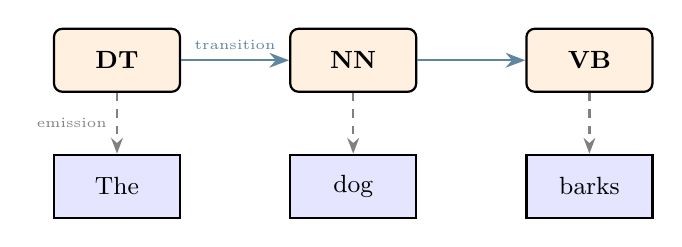
\begin{tikzpicture}[
  tag/.style={rectangle, draw, thick, fill=orange!12, minimum width=1.6cm, minimum height=0.8cm, align=center, font=\small\bfseries, rounded corners=3pt},
  wd/.style={rectangle, draw, thick, fill=blue!10, minimum width=1.6cm, minimum height=0.8cm, align=center, font=\small},
  tr/.style={-{Stealth[length=2.5mm]}, thick, primary!70},
  em/.style={-{Stealth[length=2mm]}, thick, dashed, gray}
]
  \node[tag] (t1) at (0,1.6) {DT};
  \node[tag] (t2) at (3,1.6) {NN};
  \node[tag] (t3) at (6,1.6) {VB};
  \node[wd] (w1) at (0,0) {The};
  \node[wd] (w2) at (3,0) {dog};
  \node[wd] (w3) at (6,0) {barks};
  \draw[tr] (t1) -- node[above, font=\tiny]{transition} (t2);
  \draw[tr] (t2) -- (t3);
  \draw[em] (t1) -- node[left, font=\tiny]{emission} (w1);
  \draw[em] (t2) -- (w2);
  \draw[em] (t3) -- (w3);
\end{tikzpicture}
\end{center}

\subsection{RNNs, LSTMs, and GRUs}
\begin{itemize}[leftmargin=*]
  \item \textbf{Recurrent Neural Network (RNN):} Processes a sequence one token at a time, passing a hidden state forward to remember earlier context.
  \item \textbf{Vanishing Gradient Problem:} Plain RNNs struggle to retain information over long sequences during training.
  \item \textbf{LSTM (Long Short-Term Memory):} Adds input, forget, and output gates to control what information is kept or discarded, handling long-range dependencies far better.
  \item \textbf{GRU (Gated Recurrent Unit):} A simplified alternative to LSTM with fewer gates, often just as effective and faster to train.
\end{itemize}

\subsection{Sequence-to-Sequence (Seq2Seq) Models}
\begin{conceptbox}[Seq2Seq]
A Seq2Seq model uses an \textbf{encoder} to compress an input sequence into a context representation, and a \textbf{decoder} to generate an output sequence from it --- the foundation of neural machine translation and abstractive summarization.
\end{conceptbox}

%=============================================================
\section{Attention and Transformer Architecture}
%=============================================================

\begin{definitionbox}[The Problem with RNNs]
RNNs process words one at a time and can ``forget'' distant context, and they are slow to train because they cannot be fully parallelized. The \textbf{Transformer} architecture (2017) solved both problems using \textbf{attention}.
\end{definitionbox}

\subsection{Self-Attention Mechanism}
\begin{conceptbox}[Self-Attention]
Self-attention lets every word in a sentence directly look at every other word and learn how much to ``attend to'' each one, regardless of distance, using Query (Q), Key (K), and Value (V) vectors:
$$
\text{Attention}(Q,K,V) = \text{softmax}\!\left(\frac{QK^{T}}{\sqrt{d_k}}\right)V
$$
\end{conceptbox}

\begin{center}
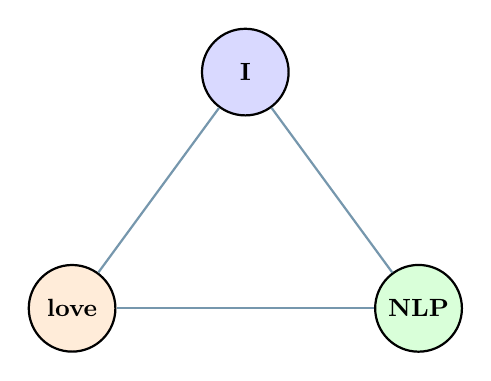
\begin{tikzpicture}
  \node[circle, draw, thick, fill=blue!15, minimum size=1.1cm, font=\bfseries\small] (w1) at (0,2) {I};
  \node[circle, draw, thick, fill=orange!15, minimum size=1.1cm, font=\bfseries\small] (w2) at (-2.2,-1) {love};
  \node[circle, draw, thick, fill=green!15, minimum size=1.1cm, font=\bfseries\small] (w3) at (2.2,-1) {NLP};
  \draw[thick, primary!60] (w1) -- (w2);
  \draw[thick, primary!60] (w2) -- (w3);
  \draw[thick, primary!60] (w3) -- (w1);
\end{tikzpicture}
\end{center}

\begin{examplebox}[Illustrative Example: Why Attention Helps]
``The animal didn't cross the street because \textit{it} was tired.'' Self-attention allows the model to strongly connect \textit{it} with \textit{animal} (not \textit{street}), correctly resolving the reference using context from anywhere in the sentence.
\end{examplebox}

\subsection{Transformer Encoder-Decoder}
\begin{center}
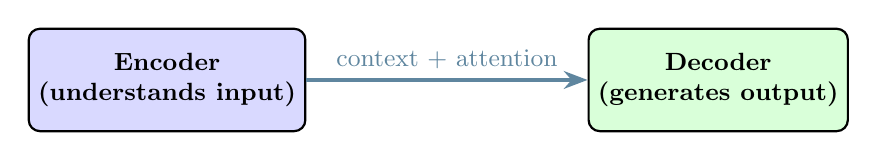
\begin{tikzpicture}[
  tbox/.style={rectangle, draw, thick, fill=#1, minimum width=3.2cm, minimum height=1.3cm, align=center, font=\small\bfseries, rounded corners=4pt},
  arr/.style={-{Stealth[length=3mm]}, very thick, line width=1.5pt}
]
  \node[tbox=blue!15] (enc) at (0,0) {Encoder\\(understands input)};
  \node[tbox=green!15] (dec) at (7,0) {Decoder\\(generates output)};
  \draw[arr, primary!70] (enc) -- node[above, font=\small] {context + attention} (dec);
\end{tikzpicture}
\end{center}

\subsection{BERT, GPT, and Large Language Models}
\rowcolors{2}{white}{defbg}
\begin{center}
\begin{tabular}{@{}p{2.6cm}p{5.3cm}p{5.3cm}@{}}
\toprule
\rowcolor{primary!15}
\textbf{Aspect} & \textbf{BERT} & \textbf{GPT} \\
\midrule
Architecture & Encoder-only & Decoder-only \\
Training Objective & Masked Language Modeling & Next-token (autoregressive) prediction \\
Context Direction & Bidirectional & Left-to-right (causal) \\
Typical Use & Classification, NER, Q\&A (understanding) & Text generation, chat (generation) \\
\bottomrule
\end{tabular}
\end{center}

\begin{conceptbox}[Large Language Models]
LLMs (e.g., GPT-4) are Transformer-based models with billions of parameters, trained on massive text corpora, capable of few-shot learning: performing new tasks from just a few examples in the prompt, without retraining.
\end{conceptbox}

%=============================================================
\section{Core NLP Tasks and Applications}
%=============================================================

\subsection{Common NLP Tasks}
\begin{itemize}[leftmargin=*]
  \item \textbf{Text Classification:} Assigning a category to a document (e.g., spam vs.\ not spam).
  \item \textbf{Sentiment Analysis:} Determining whether text expresses positive, negative, or neutral opinion.
  \item \textbf{Machine Translation:} Automatically translating text from one language to another.
  \item \textbf{Text Summarization:} \textit{Extractive} (selecting key sentences) or \textit{Abstractive} (generating new, condensed sentences).
  \item \textbf{Question Answering:} Automatically producing an answer to a natural-language question, often from a given passage.
  \item \textbf{Chatbots and Dialogue Systems:} Maintaining multi-turn conversations with users.
  \item \textbf{Topic Modeling:} Discovering abstract topics in a collection of documents (e.g., Latent Dirichlet Allocation, LDA).
\end{itemize}

\subsection{Applications of NLP}
\rowcolors{2}{white}{defbg}
\begin{longtable}{@{}p{3.5cm}p{10cm}@{}}
\toprule
\rowcolor{primary!15}
\textbf{Domain} & \textbf{Example Applications} \\
\midrule
\endhead
Healthcare & Clinical note analysis, symptom extraction, medical Q\&A. \\
\addlinespace
Business \& IT & Customer sentiment analysis, support chatbots, email spam filters. \\
\addlinespace
Search Engines & Query understanding, semantic search, result ranking. \\
\addlinespace
Translation Services & Real-time machine translation (e.g., Google Translate). \\
\addlinespace
Legal & Contract review, e-discovery, case-law search. \\
\addlinespace
Education & Automated essay scoring, plagiarism detection, tutoring chatbots. \\
\addlinespace
Social Media & Content moderation, trend and misinformation detection. \\
\bottomrule
\end{longtable}

%=============================================================
\section{Speech Processing Basics}
%=============================================================

\begin{definitionbox}[Speech Processing]
Speech processing connects NLP with spoken language, converting between audio signals and text so that voice assistants and dictation tools can understand and respond to spoken input.
\end{definitionbox}

\subsection{Automatic Speech Recognition (ASR)}
\begin{conceptbox}[ASR]
ASR (speech-to-text) converts an audio waveform into text, typically using an acoustic model (mapping sound to phonemes) combined with a language model (choosing the most likely word sequence).
\end{conceptbox}

\subsection{Text-to-Speech (TTS)}
\begin{conceptbox}[TTS]
TTS (speech synthesis) converts written text into natural-sounding spoken audio, used in voice assistants, screen readers, and accessibility tools.
\end{conceptbox}

\begin{itemize}[leftmargin=*]
  \item \textbf{Word Error Rate (WER):} The standard metric for ASR accuracy, measuring insertions, deletions, and substitutions relative to a reference transcript.
  \item \textbf{Applications:} Voice assistants (Siri, Alexa), automated transcription, accessibility tools, and voice-controlled IoT devices.
\end{itemize}

%=============================================================
\section{Evaluation Metrics in NLP}
%=============================================================

\begin{definitionbox}[Why Evaluate?]
Different NLP tasks need different evaluation metrics --- classification accuracy is meaningless for translation quality, and vice versa.
\end{definitionbox}

\subsection{Classification Metrics (Recap)}
For tasks like spam detection or sentiment classification:
$$
\text{Accuracy}=\frac{TP+TN}{TP+TN+FP+FN}, \quad
\text{Precision}=\frac{TP}{TP+FP}, \quad
\text{Recall}=\frac{TP}{TP+FN}, \quad
F1=2\cdot\frac{P\cdot R}{P+R}
$$

\subsection{BLEU Score (Machine Translation)}
\begin{conceptbox}[BLEU]
BLEU (Bilingual Evaluation Understudy) compares a machine-generated translation to one or more human reference translations by measuring \textbf{n-gram precision} (how many candidate n-grams appear in the reference), combined with a \textbf{brevity penalty} that discourages overly short outputs.
\end{conceptbox}

\subsection{ROUGE Score (Summarization)}
\begin{conceptbox}[ROUGE]
ROUGE (Recall-Oriented Understudy for Gisting Evaluation) measures how much n-gram content from the human reference summary is \textbf{recalled} by the machine-generated summary --- the complementary counterpart to BLEU's precision focus.
\end{conceptbox}

\subsection{Perplexity (Recap)}
Lower perplexity $PP(W)=P(w_1,\ldots,w_N)^{-1/N}$ indicates a language model assigns higher probability to real text, i.e., it models the language better.

%=============================================================
\section{Ethical and Responsible NLP}
%=============================================================

\begin{alertbox}[Key Concerns]
As NLP systems (especially LLMs) are deployed widely, BSIT professionals must understand their risks and responsibilities.
\end{alertbox}

\begin{itemize}[leftmargin=*]
  \item \textbf{Bias:} Models can learn and amplify gender, racial, or cultural biases present in training text (e.g., biased word embeddings or stereotyped generations).
  \item \textbf{Hallucination / Misinformation:} LLMs can generate fluent but factually incorrect or fabricated content with high confidence.
  \item \textbf{Privacy:} Models trained on large text corpora may memorize and leak sensitive personal information.
  \item \textbf{Toxic Content Generation:} Language models can be prompted to produce harmful, offensive, or abusive text if not properly safeguarded.
  \item \textbf{Copyright and Data Provenance:} Training on copyrighted text raises unresolved legal and ethical questions.
  \item \textbf{Job Impact:} Automation of translation, transcription, and customer support may displace certain roles, requiring reskilling.
\end{itemize}

\begin{conceptbox}[Responsible NLP Principles]
Fairness $\bullet$ Reliability and Safety $\bullet$ Privacy and Security $\bullet$ Inclusiveness $\bullet$ Transparency $\bullet$ Accountability.
\end{conceptbox}

%=============================================================
\section{Core Mathematical Foundations for NLP}
%=============================================================

\subsection{Probability Recap}
\begin{itemize}[leftmargin=*]
  \item \textbf{Conditional Probability:} $P(A\mid B)=\dfrac{P(A\cap B)}{P(B)}$, the basis of n-gram and HMM models.
  \item \textbf{Bayes' Theorem:} $P(A\mid B)=\dfrac{P(B\mid A)P(A)}{P(B)}$, the foundation of Naive Bayes text classification.
  \item \textbf{Chain Rule:} $P(w_1,\ldots,w_n)=\prod_{i=1}^n P(w_i\mid w_1,\ldots,w_{i-1})$, the basis of all language models.
\end{itemize}

\subsection{Why Use Log Probabilities?}
\begin{conceptbox}[Avoiding Numerical Underflow]
Multiplying many small probabilities together (as in long sentences) quickly underflows to zero on a computer. NLP systems instead sum \textbf{log probabilities}:
$$
\log P(w_1,\ldots,w_n) = \sum_{i=1}^{n}\log P(w_i \mid w_{i-1})
$$
\end{conceptbox}

\subsection{Vectors and Similarity Recap}
Text representation, introduced earlier, converts words/documents into vectors $\mathbf{A}, \mathbf{B}$; similarity is then computed using the dot product $\mathbf{A}\cdot\mathbf{B}=\sum_i A_iB_i$ and cosine similarity, which underlie nearly all modern retrieval, clustering, and recommendation over text.

%=============================================================
\section{Exam-Oriented Worked Examples}
%=============================================================

\begin{examplebox}[Worked Example 1: Bigram Probability from a Mini Corpus]
Training corpus: ``I love NLP'', ``I love AI'', ``I love data''.\\
Counts: $\text{Count(I)}=3$, $\text{Count(I, love)}=3$, $\text{Count(love)}=3$, $\text{Count(love, NLP)}=1$.
$$
P(\text{love}\mid \text{I}) = \frac{\text{Count(I, love)}}{\text{Count(I)}} = \frac{3}{3} = 1.0
$$
$$
P(\text{NLP}\mid \text{love}) = \frac{\text{Count(love, NLP)}}{\text{Count(love)}} = \frac{1}{3} \approx 0.33
$$
\end{examplebox}

\begin{examplebox}[Worked Example 2: TF-IDF Computation]
A document has 50 total words; the term ``data'' appears 5 times, so $TF=5/50=0.1$. The corpus has $N=100$ documents, and ``data'' appears in $df=10$ of them:
$$
IDF = \log_{10}\frac{100}{10} = \log_{10}(10) = 1
$$
$$
TF\text{-}IDF = 0.1 \times 1 = 0.1
$$
\end{examplebox}

\begin{examplebox}[Worked Example 3: Cosine Similarity]
Given vectors $\mathbf{A}=(1,2,3)$ and $\mathbf{B}=(2,3,1)$:
$$
\mathbf{A}\cdot\mathbf{B} = (1)(2)+(2)(3)+(3)(1) = 2+6+3 = 11
$$
$$
\lVert \mathbf{A}\rVert = \lVert \mathbf{B}\rVert = \sqrt{1^2+2^2+3^2}=\sqrt{14}
$$
$$
\cos(\theta) = \frac{11}{\sqrt{14}\times\sqrt{14}} = \frac{11}{14} \approx 0.786
$$
The vectors are fairly similar (close to 1).
\end{examplebox}

\begin{examplebox}[Worked Example 4: Edit (Levenshtein) Distance]
Transform ``kitten'' into ``sitting'':
\begin{itemize}[leftmargin=*]
  \item \textbf{kitten} $\to$ \textbf{sitten} (substitute k $\to$ s)
  \item \textbf{sitten} $\to$ \textbf{sittin} (substitute e $\to$ i)
  \item \textbf{sittin} $\to$ \textbf{sitting} (insert g)
\end{itemize}
Total edit distance $=3$.
\end{examplebox}

\begin{examplebox}[Worked Example 5: Naive Bayes Text Classification]
Classify an email containing the word ``offer'' as spam or ham, given $P(\text{spam})=P(\text{ham})=0.5$, $P(\text{offer}\mid\text{spam})=0.6$, $P(\text{offer}\mid\text{ham})=0.1$:
$$
P(\text{spam}\mid\text{offer}) \propto 0.5 \times 0.6 = 0.30
$$
$$
P(\text{ham}\mid\text{offer}) \propto 0.5 \times 0.1 = 0.05
$$
Since $0.30 > 0.05$, classify the email as \textbf{spam} (normalized confidence $\approx 85.7\%$).
\end{examplebox}

\begin{examplebox}[Worked Example 6: Perplexity of a Language Model]
A bigram model assigns a test sentence of $N=5$ words a total probability $P=0.001=10^{-3}$:
$$
PP(W) = P^{-\frac{1}{N}} = \left(10^{-3}\right)^{-\frac{1}{5}} = 10^{0.6} \approx 3.98
$$
A lower perplexity (closer to 1) would indicate an even better-fitting model.
\end{examplebox}

\begin{examplebox}[Worked Example 7: Ranking Documents by Cosine Similarity]
Query vector $\mathbf{Q}=(1,1,0)$; document vectors $\mathbf{D_1}=(2,0,1)$ and $\mathbf{D_2}=(1,1,1)$:
$$
\cos(Q,D_1) = \frac{(1)(2)+(1)(0)+(0)(1)}{\sqrt{2}\sqrt{5}} = \frac{2}{\sqrt{10}} \approx 0.632
$$
$$
\cos(Q,D_2) = \frac{(1)(1)+(1)(1)+(0)(1)}{\sqrt{2}\sqrt{3}} = \frac{2}{\sqrt{6}} \approx 0.816
$$
Since $0.816 > 0.632$, the search engine ranks $D_2$ above $D_1$ for this query.
\end{examplebox}

\begin{examplebox}[Worked Example 8: Regex Pattern Matching]
Text: ``Call 555-1234 or 555-5678 for support.'' Pattern: \texttt{\textbackslash d\{3\}-\textbackslash d\{4\}}.\\
The pattern matches two substrings, \texttt{555-1234} and \texttt{555-5678} --- showing how regex extracts structured patterns (like phone numbers) from unstructured text without training any model.
\end{examplebox}

%=============================================================
\section{Quick Revision Glossary}
%=============================================================

\rowcolors{2}{white}{defbg}
\begin{longtable}{@{}p{3.3cm}p{10.2cm}@{}}
\toprule
\rowcolor{primary!15}
\textbf{Term} & \textbf{One-Line Meaning} \\
\midrule
\endhead
Tokenization & Splitting text into words, sub-words, or sentences. \\
\addlinespace
Stemming & Rule-based chopping of word endings to an approximate root. \\
\addlinespace
Lemmatization & Dictionary/grammar-based reduction of a word to its true root (lemma). \\
\addlinespace
Stopwords & Very common, low-information words often removed before analysis. \\
\addlinespace
POS Tagging & Assigning a grammatical category to each word in a sentence. \\
\addlinespace
Parsing & Analyzing a sentence's grammatical structure (constituency or dependency). \\
\addlinespace
Corpus & A large, structured collection of text used to train/evaluate NLP models. \\
\addlinespace
N-gram & A contiguous sequence of $n$ words used to model local context. \\
\addlinespace
Markov Assumption & A word depends only on a limited number of preceding words. \\
\addlinespace
Smoothing & Reserving probability mass for unseen n-grams (e.g., Laplace smoothing). \\
\addlinespace
Perplexity & Measures how well a language model predicts test text; lower is better. \\
\addlinespace
Bag-of-Words & Document representation as word counts, ignoring order. \\
\addlinespace
TF-IDF & Term weighting that balances term frequency against document frequency. \\
\addlinespace
Word Embedding & Dense vector representation of a word capturing semantic meaning. \\
\addlinespace
Word2Vec & Neural method (CBOW/Skip-gram) for learning word embeddings. \\
\addlinespace
Cosine Similarity & Similarity between two vectors based on the angle between them. \\
\addlinespace
NER & Identifying and classifying named entities (person, org, location, date). \\
\addlinespace
WSD & Determining which meaning of an ambiguous word applies in context. \\
\addlinespace
Semantic Role Labeling & Labeling ``who did what to whom, when, and where'' in a sentence. \\
\addlinespace
HMM & Probabilistic model using hidden states (tags) and observations (words). \\
\addlinespace
Self-Attention & Mechanism letting each word weigh the relevance of every other word. \\
\addlinespace
Transformer & Attention-based architecture underlying BERT, GPT, and modern LLMs. \\
\addlinespace
BERT & Encoder-only Transformer trained via masked language modeling. \\
\addlinespace
GPT & Decoder-only Transformer trained to predict the next token. \\
\addlinespace
BLEU Score & Precision-based metric for evaluating machine translation quality. \\
\addlinespace
ROUGE Score & Recall-based metric for evaluating automatic text summarization. \\
\addlinespace
Regular Expression & A pattern that compactly describes a set of matching strings, used for extraction. \\
\addlinespace
Finite-State Automaton (FSA) & A simple machine with states and transitions, used for rule-based morphology. \\
\addlinespace
Inverted Index & A mapping from each term to the documents containing it, enabling fast search. \\
\addlinespace
Vector Space Model & Represents documents/queries as vectors, ranked by cosine similarity for retrieval. \\
\addlinespace
Coreference Resolution & Linking pronouns and noun phrases that refer to the same real-world entity. \\
\addlinespace
ASR & Automatic Speech Recognition; converts spoken audio into text. \\
\addlinespace
TTS & Text-to-Speech; converts written text into spoken audio. \\
\bottomrule
\end{longtable}

%=============================================================
\section{Question Bank Blueprint (80 Marks Support)}
%=============================================================

\begin{conceptbox}[Suggested 80 Marks Distribution]
\begin{itemize}[leftmargin=*]
  \item \textbf{Section A:} MCQs and definitions (20 marks)
  \item \textbf{Section B:} Short conceptual questions (20 marks)
  \item \textbf{Section C:} Descriptive/theory questions (20 marks)
  \item \textbf{Section D:} Numerical/problem-solving questions (20 marks)
\end{itemize}
\end{conceptbox}

\subsection{Important Theory Questions}
\begin{itemize}[leftmargin=*]
  \item Explain the different levels of language analysis with examples.
  \item Differentiate stemming and lemmatization with examples.
  \item Describe the complete NLP preprocessing pipeline using a sample sentence.
  \item Explain how regular expressions and finite-state automata are used in NLP.
  \item Differentiate constituency parsing and dependency parsing.
  \item Explain the Markov assumption used in n-gram language models.
  \item Explain why smoothing is necessary in language modeling.
  \item Differentiate Bag-of-Words, TF-IDF, and word embeddings as text representations.
  \item Explain Word2Vec, contrasting the CBOW and Skip-gram approaches.
  \item Explain the vector space model and how an inverted index speeds up search.
  \item Differentiate Named Entity Recognition, Word Sense Disambiguation, and Coreference Resolution.
  \item Explain the self-attention mechanism and why Transformers replaced RNNs.
  \item Differentiate BERT and GPT in terms of architecture and typical use.
  \item Differentiate Automatic Speech Recognition (ASR) and Text-to-Speech (TTS).
  \item Discuss ethical issues in NLP such as bias, hallucination, and privacy.
\end{itemize}

\subsection{Important Numerical/Analytical Questions}
\begin{itemize}[leftmargin=*]
  \item Compute a bigram probability given word and bigram counts from a small corpus.
  \item Compute TF-IDF for a term given its frequency and corpus statistics.
  \item Compute cosine similarity between two given word/document vectors.
  \item Rank two documents against a query using cosine similarity.
  \item Compute the edit (Levenshtein) distance between two short strings.
  \item Given a short text and a regex pattern, identify all matching substrings.
  \item Classify a test document using Naive Bayes given simple probability tables.
  \item Compute the perplexity of a language model given a test sequence probability.
\end{itemize}

\subsection{Sample MCQs with Answer Key}
\begin{enumerate}[leftmargin=*]
  \item Which process can map ``better'' to its lemma ``good'' using vocabulary and grammar knowledge?\\
  (a) Stemming \quad (b) Lemmatization \quad (c) Tokenization \quad (d) Parsing
  \item Which formula represents Term Frequency--Inverse Document Frequency weighting?\\
  (a) $TF \times IDF$ \quad (b) $TF + IDF$ \quad (c) $TF / IDF$ \quad (d) $IDF - TF$
  \item In the Transformer architecture, which mechanism lets the model relate words regardless of distance?\\
  (a) Convolution \quad (b) Pooling \quad (c) Self-Attention \quad (d) Backpropagation
  \item Which metric is most commonly used to evaluate machine translation quality?\\
  (a) Accuracy \quad (b) BLEU \quad (c) Perplexity \quad (d) Entropy
  \item BERT is best described as a:\\
  (a) Decoder-only autoregressive model \quad (b) Encoder-only bidirectional model \quad (c) Rule-based grammar checker \quad (d) Purely statistical n-gram model
  \item Which NLP task involves identifying names of people, organizations, and locations in text?\\
  (a) POS Tagging \quad (b) Named Entity Recognition \quad (c) Text Summarization \quad (d) Stemming
  \item Lower perplexity on a test set indicates:\\
  (a) A worse language model \quad (b) A better language model \quad (c) No relationship to model quality \quad (d) Overfitting only
  \item Which data structure allows a search engine to instantly find documents containing a query term?\\
  (a) Parse tree \quad (b) Inverted index \quad (c) Confusion matrix \quad (d) Embedding matrix
  \item Coreference resolution is primarily concerned with:\\
  (a) Assigning POS tags \quad (b) Linking expressions that refer to the same entity \quad (c) Measuring translation quality \quad (d) Compressing word vectors
\end{enumerate}
\begin{conceptbox}[Answer Key]
1--(b), 2--(a), 3--(c), 4--(b), 5--(b), 6--(b), 7--(b), 8--(b), 9--(b)
\end{conceptbox}

%=============================================================
\section{Summary}
%=============================================================

\begin{examplebox}[Key Takeaways]
\begin{itemize}[leftmargin=*]
  \item NLP enables machines to process human language across phonological, morphological, syntactic, semantic, pragmatic, and discourse levels.
  \item Text preprocessing, regular expressions, and finite-state methods provide the rule-based foundation of every NLP pipeline.
  \item N-gram language models use the Markov assumption, smoothing, and perplexity to model word sequences probabilistically.
  \item Text representation has evolved from Bag-of-Words and TF-IDF to dense word embeddings and contextual Transformer representations, underpinning information retrieval via the vector space model.
  \item Semantic analysis (WSD, NER, SRL, coreference resolution) and sequence models (HMM, RNN, LSTM) extract meaning and structure from language.
  \item Attention and Transformers (BERT, GPT, LLMs) are the foundation of modern state-of-the-art NLP, complemented by speech processing (ASR/TTS) for spoken language.
  \item Task-appropriate evaluation (accuracy/F1, BLEU, ROUGE, perplexity) and responsible, ethical use are essential for real-world NLP systems.
\end{itemize}
\end{examplebox}

\end{document}
